\ifnum\pdfoutput=0
  \def\pgfsysdriver{pgfsys-dvisvgm.def}
\fi
\documentclass[tikz,border=0pt]{standalone}
\usepackage{tikz}
\usetikzlibrary{arrows.meta}
\usepackage[scaled=0.92]{helvet}
\renewcommand{\familydefault}{\sfdefault}

% Colors matching blog _variables.scss and diagram palette
\definecolor{bg}{HTML}{1E1E1E}
\definecolor{treeline}{HTML}{BEBEBE}
\definecolor{digitcolor}{HTML}{D9D9D9}
\definecolor{swapcyan}{HTML}{19D4FA}

\newcommand{\drawtree}[1]{
    % Outer triangle and internal binary tree branches
    % Using round caps and joins ensures all T-junctions and box-top attachments
    % are completely flush without protruding corners.
    \draw[treeline, line width=2.2pt, line join=round, line cap=round]
        (#1 + 0.5, 0) -- (#1 + 4.0, 5.3375) -- (#1 + 7.5, 0)
        (#1 + 3.5, 0) -- (#1 + 2.0, 2.2875)
        (#1 + 4.5, 0) -- (#1 + 6.0, 2.2875)
        (#1 + 1.5, 0) -- (#1 + 1.0, 0.7625)
        (#1 + 2.5, 0) -- (#1 + 3.0, 0.7625)
        (#1 + 5.5, 0) -- (#1 + 5.0, 0.7625)
        (#1 + 6.5, 0) -- (#1 + 7.0, 0.7625);
    % Array outer box (drawn with -- cycle so dvisvgm emits a single M ... L ... Z path)
    \draw[treeline, line width=2.2pt, line join=miter]
        (#1, -1) -- (#1 + 8, -1) -- (#1 + 8, 0) -- (#1, 0) -- cycle;
    % Array vertical cell dividers
    \foreach \i in {1,...,7} {
        \draw[treeline, line width=2.2pt] (#1 + \i, -1) -- (#1 + \i, 0);
    }
}

\begin{document}
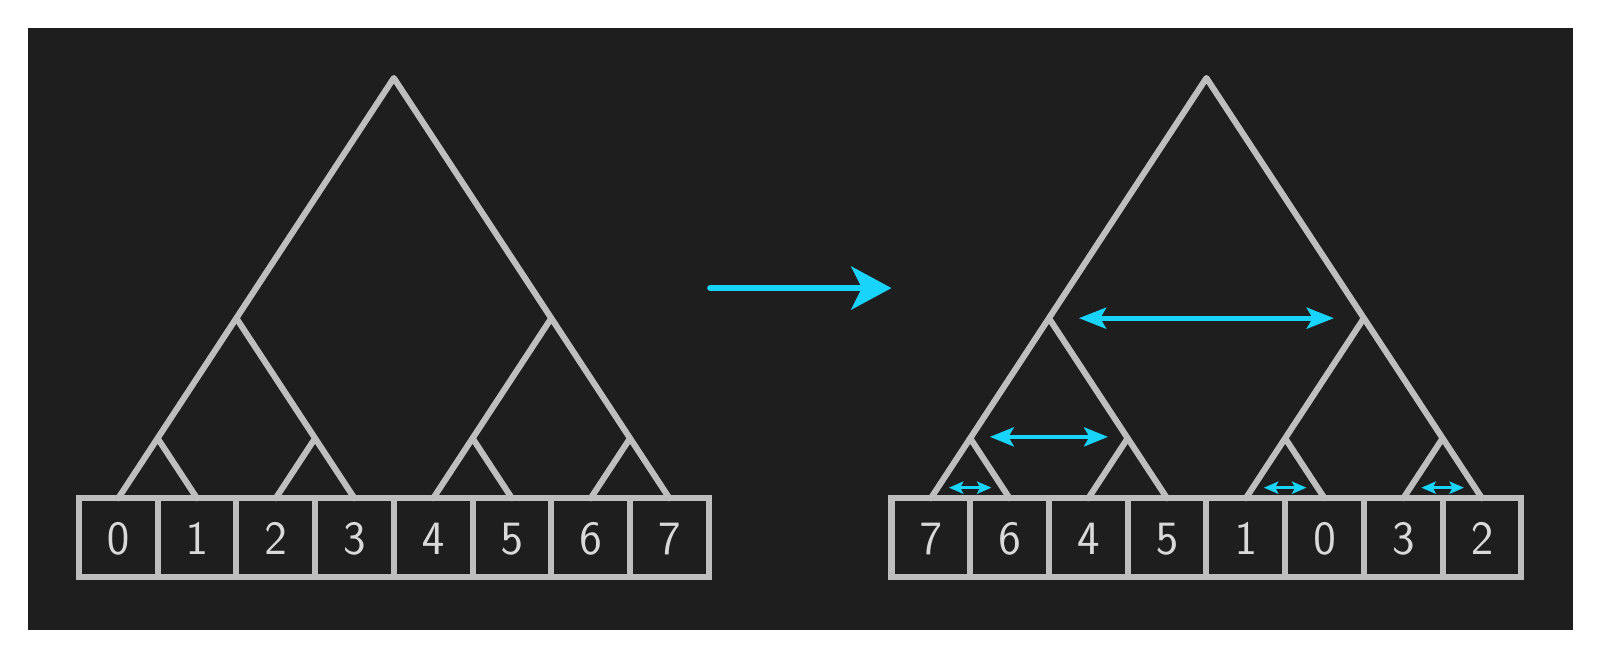
\begin{tikzpicture}[x=1cm, y=1cm]
    % Total width: -0.65 to 18.97 (19.62 units), height: -1.675 to 5.977 (7.652 units)
    % Aspect ratio: 19.62 / 7.6518 = 2.5641 (800 x 312)
    \path[use as bounding box] (-0.65, -1.675) rectangle (18.97, 5.977);
    \fill[bg] (-0.65, -1.675) rectangle (18.97, 5.977);

    % Left unshuffled tree & array [0..7]
    \drawtree{0}
    \foreach \i/\val in {0/0, 1/1, 2/2, 3/3, 4/4, 5/5, 6/6, 7/7} {
        \node[color=digitcolor, font=\fontsize{19}{19}\selectfont, anchor=center]
            at (\i + 0.5, -0.52) {\val};
    }

    % Center transition arrow
    \draw[swapcyan, line width=2.3pt, line cap=round,
          -{Stealth[length=14.5pt, width=15.5pt, inset=3.8pt]}]
        (8.02, 2.67) -- (10.32, 2.67);

    % Right Owen-scrambled tree & array [7, 6, 4, 5, 1, 0, 3, 2]
    \def\rx{10.32}
    \drawtree{\rx}
    \foreach \i/\val in {0/7, 1/6, 2/4, 3/5, 4/1, 5/0, 6/3, 7/2} {
        \node[color=digitcolor, font=\fontsize{19}{19}\selectfont, anchor=center]
            at (\rx + \i + 0.5, -0.52) {\val};
    }

    % Swap arrows inside the right tree
    % Level 3 (top: swapping the two halves of size 4)
    \draw[swapcyan, line width=1.9pt,
          {Stealth[length=9.8pt, width=7.5pt, inset=2.1pt]}-{Stealth[length=9.8pt, width=7.5pt, inset=2.1pt]}]
        (\rx + 2.38, 2.2875) -- (\rx + 5.62, 2.2875);

    % Level 2 (middle left: swapping the left two pairs of size 2)
    \draw[swapcyan, line width=1.7pt,
          {Stealth[length=8.6pt, width=6.8pt, inset=1.9pt]}-{Stealth[length=8.6pt, width=6.8pt, inset=1.9pt]}]
        (\rx + 1.25, 0.78) -- (\rx + 2.75, 0.78);

    % Level 1 (bottom pairs: swapping leaf pairs 0, 2, 3)
    \foreach \cx in {1.0, 5.0, 7.0} {
        \draw[swapcyan, line width=1.15pt,
              {Stealth[length=5.2pt, width=4.4pt, inset=1.1pt]}-{Stealth[length=5.2pt, width=4.4pt, inset=1.1pt]}]
            (\rx + \cx - 0.27, 0.135) -- (\rx + \cx + 0.27, 0.135);
    }
\end{tikzpicture}
\end{document}
